The analysis presented so far has been able to fully characterise the behaviour of the space-homogeneous kinetic model. However, it is unable to describe the dynamics of the full space-inhomogeneous model. It has been shown that the space-homogeneous model possesses only three invariant measures and converges to one of them dependent on the sign of the mean of the initial data. The full model also has these invariant measures, however it is not proven whether these are all of them or not. That is, the full model may have stationary distributions which are not homogeneous in space. By utilising numerical methods, we can relax some of the restrictions which the analysis requires. The goal is to show that for some choice of initial data and interaction function, the particle system will have a stationary distribution that isn't uniform in space. At its most basic, this could be two clusters of particles moving on the same direction diametrically opposite each other. The system will still converge in velocity to the values predicted by the homogeneous model, but spatial heterogeneity will remain. While this may be the case for the particle system, we conjecture that such behaviour will not occur in the kinetic model.

The aim is to be able to accurately simulate the dynamics of both the space-inhomogeneous PDE +++ref+++ and the corresponding interacting particle system. The latter is relatively simple to simulate using techniques for SDEs. However, we have shown analytically that the particle system does not have the same invariant measures as the continuum model, or indeed its McKean-Vlasov equation. The kinetic model is more difficult as it contains both advective and diffusive terms. We begin this section with a presentation of numerical methods for SDEs before reviewing methods for advection-type and diffusion-type equations, following the treatment of Hundsdorfer and Verwer \cite{Hundsdorfer2007} as well as Morton and Meyers \cite{Morton2005}.

Mirroring the approach in the analysis, we will develop the techniques required first for the space-homogeneous system with no interaction, before adding further levels of complexity. Doing so allows the rigorous testing of any schemes developed as analytic solutions are available. Throughout this section it is recommended to follow along with the supplementary Jupyter notebook available at: 
 %\url{https://github.com/Tom271/Whales} +++Change name+++
Every figure within this report was produced using the notebook and its accompanying source code.

\subsection{Particle Systems}\label{sec:homparticlesystem}
Simulating particle systems requires the numerical solution of coupled SDEs. The standard method for this is the Euler-Maruyama (EM) method, which can be seen as the stochastic analogue of Euler's method. Our motivating example here will be the Ornstein-Uhlenbeck process\footnote{This is also the overdamped Langevin equation}. 
\begin{equation}
\dif x_t = - x_t \dif t + \sigma \dif W_t
\end{equation}
This is exactly the same evolution as that which drives the space-homogeneous particle system \eqref{eq:homparticle}, with no interaction between particles, and so provides the ideal starting point. It describes the motion of a damped particle moving randomly within a potential well as illustrated in Section \ref{sec:particledynamics}. Applying the EM method to the above equation gives:
\[ x_{n+1} = x_n -  x_n\Dt + \sqrt{2\sigma\Dt}Z_n,  \]
where $Z_n$ is a standard normal random variable. This discretisation is very quick to compute, and has strong order $\frac{1}{2}$ \cite{Higham01}. This gives us a method of finding the stationary distribution: simulate many particles for a long time. Eventually, the density of the particles will be approximately the stationary distribution of the system. In this case it is in fact not even necessary to simulate many particles -- if the system is allowed to evolve for long enough, one particle will suffice as there is no interaction between particles and the scheme is ergodic. The particle system will be an excellent metric by which to test the schemes developed for the continuum models. One drawback however will be the presence of only one invariant measure, as was shown analytically in Section \ref{sec:particledynamics} and will be shown numerically in Section \ref{sec:homparticles}.
\begin{figure}
    \centering
    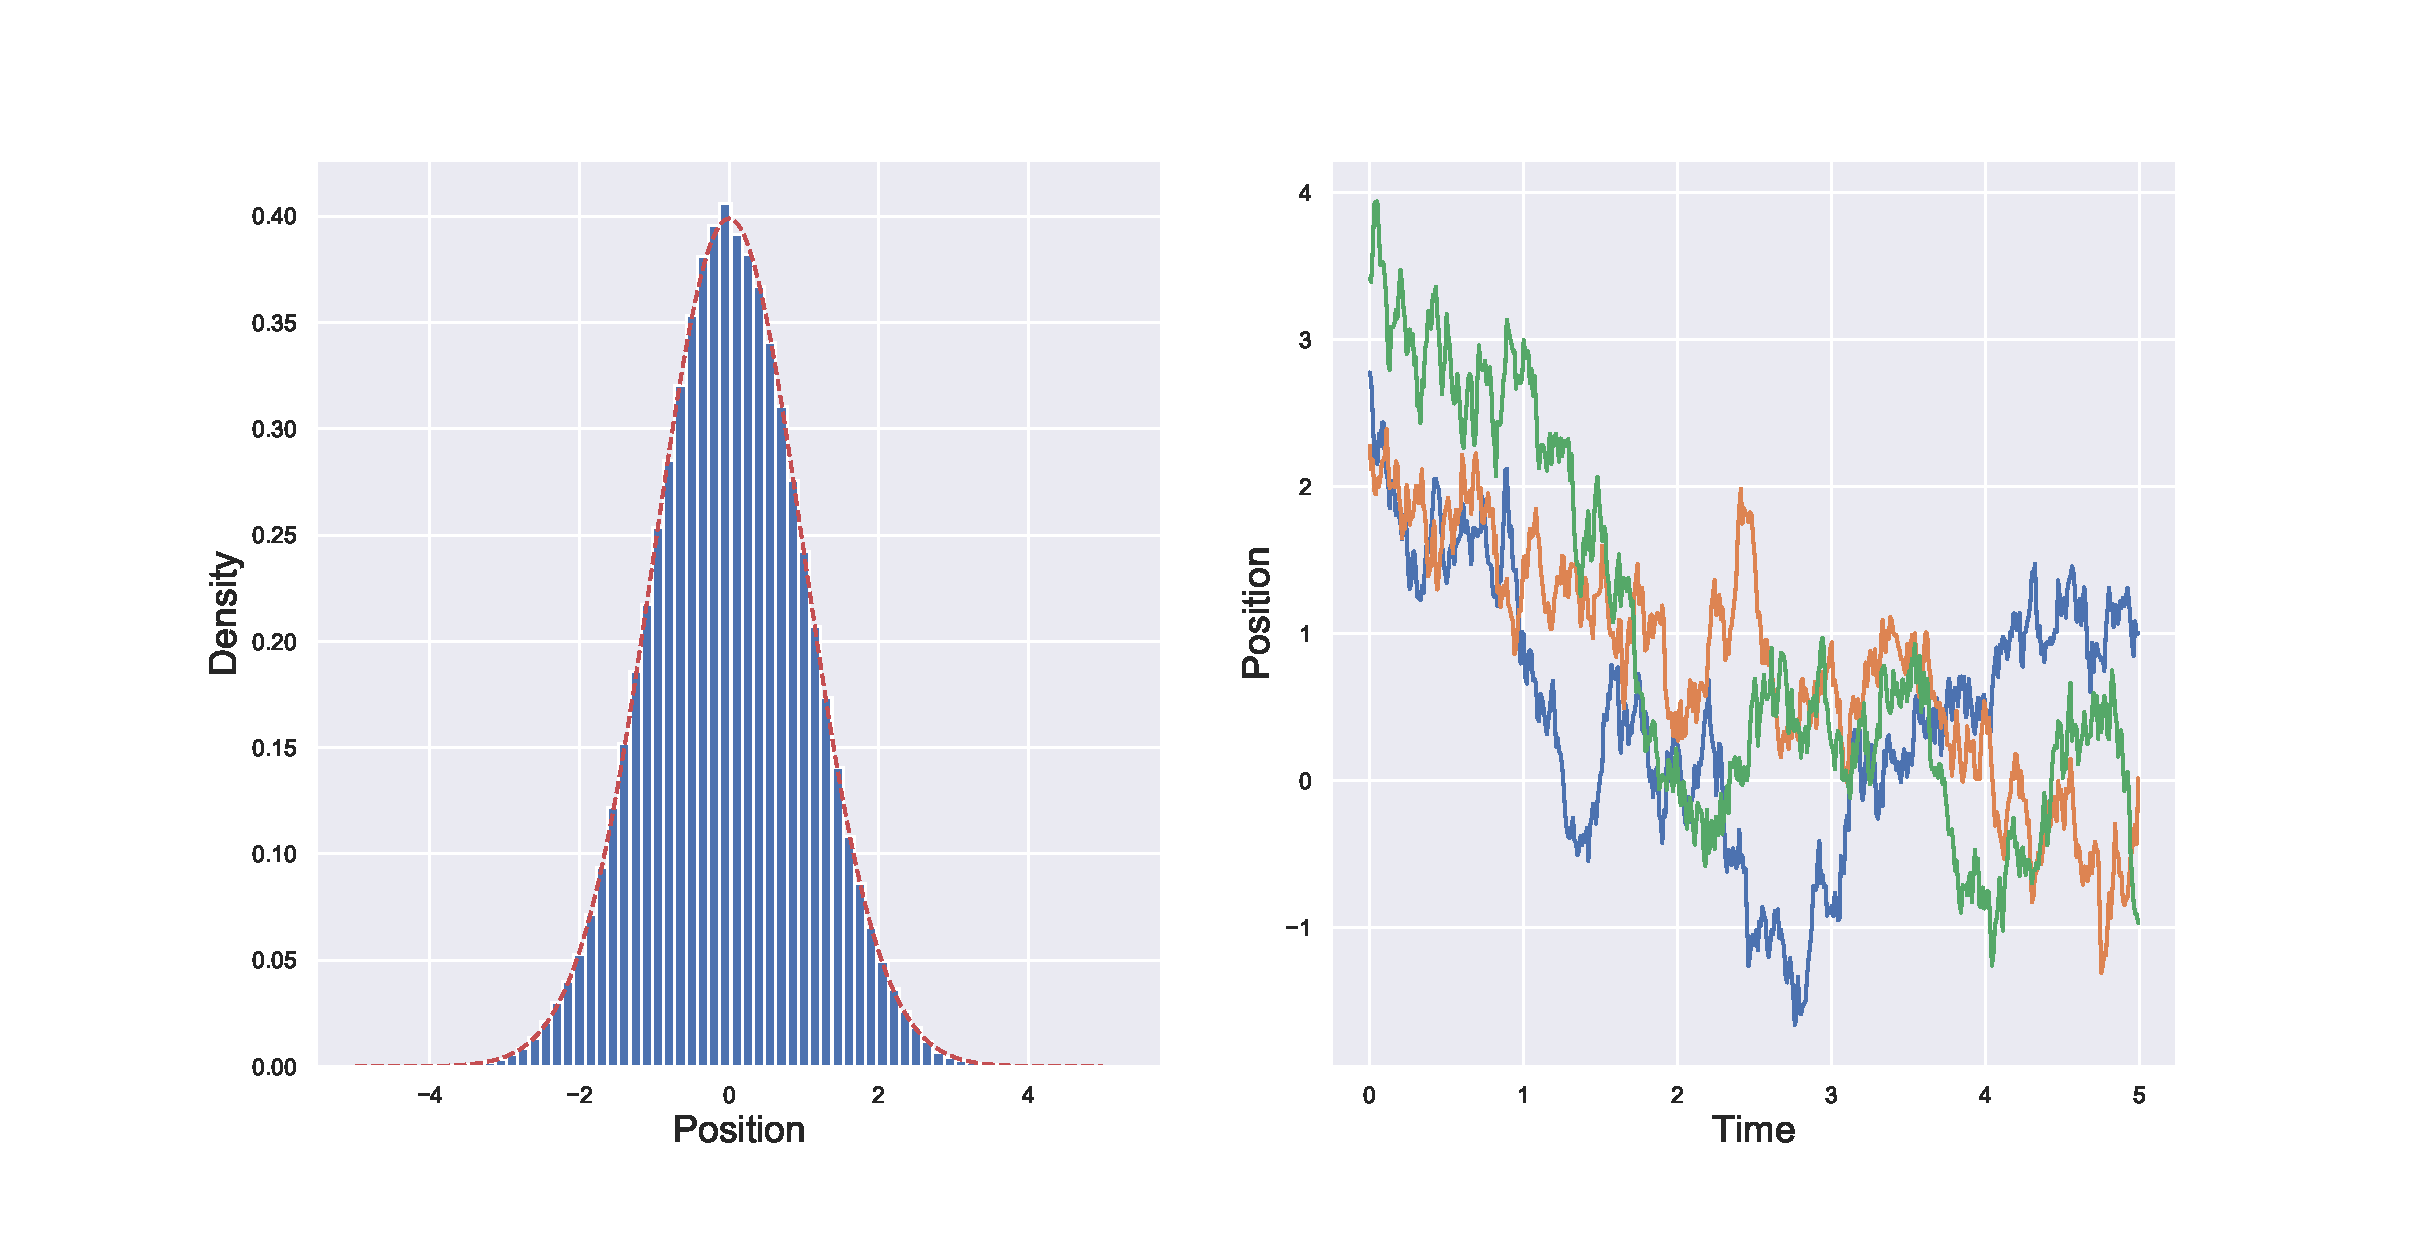
\includegraphics[width=\linewidth]{Figures/OUparticletraj}
    \caption{Histogram of positions of 1000 particles after 100s with $\sigma = 1$, and positions of 5 particles over time. +++conv in moments?+++}
    \label{fig:ouparticletraj}
\end{figure}

\subsection{Diffusion Equations}
As a prototypical example of a diffusion equation, consider the heat equation in one dimension given by 
\begin{equation}\label{eq:heat}
\begin{cases}
    \partial_t u(t,x) = \sigma\partial_{xx} u(t,x),&\sigma >0\\
        u(0,x) = u_0(x),  &t\in\R^+, x\in\R,
\end{cases}
\end{equation}
To solve this numerically, we must truncate the domain in both time and space. To do this, a region is chosen where we expect most of the mass to be throughout the time of interest. Here, we truncate to \(x \in [-L,L], t \in [0,T]\) for some \(L>0\) and a finite time horizon \(T\). Doing so requires a boundary condition to be enforced. A natural choice for this equation is a zero Dirichlet condition, \(u(t,L) = u(t,-L) = 0\). As long as \(L\) is chosen large enough, the heat which spreads beyond this limit is negligible -- this will however be a source of error. To mitigate this, one could compare the difference between analytic solutions (where available) on the full real line and the truncated domain, then choosing $L$ accordingly. In general, boundary conditions are determined by the phenomenon being modelled. The problem geometry may naturally suggest conditions, or they may be enforced by numerical constraints as in this case. We must also discretise in space and time, to create a mesh covering \(\left[0,T\right] \times \left[-L,L\right]\). Let \(\lbrace x_j\rbrace_{j=0}^J\) partition the space equally such that \(x_0 = -L, x_J=L\) and \(x_j-x_{j-1} = \Delta x\) for all \(j\). Similarly, let \(\lbrace t_n\rbrace_{n=0}^N\) partition \(\left[0,T\right]\) in such a way that \(t_0=0, t_N =T\) and \(t_n-t_{n-1} = \Delta t\). The parameters \(\Delta x, \Delta t\) are the space step and time step respectively. We thus have a discretised description of the continuum that we can implement. 

\subsubsection*{Forward Time Centred Space}
The aim is to solve the equation approximately on this grid. We shall denote approximate solutions by capital letters, that is \(u(x_j,t_n) \approx U_j^n\). How can we approximate the solution? We must approximate each term in the equation separately. First the time derivative, or transient term can be approximated using the definition of the derivative. Recall
\[
\od{u}{t} = \lim_{\Delta t \to 0}\frac{u(t+\Dt) - u(t)}{\Dt}.
\]
We can then approximate the time derivative for fixed $x$ by simply taking \(\Dt\) small. Doing so leads to the forward difference approximation
\[
\partial_t u(t_n,x_j) \approx \frac{U^{n+1}_j- U^n_j}{\Dt}.
\]
\begin{figure}
    \centering
    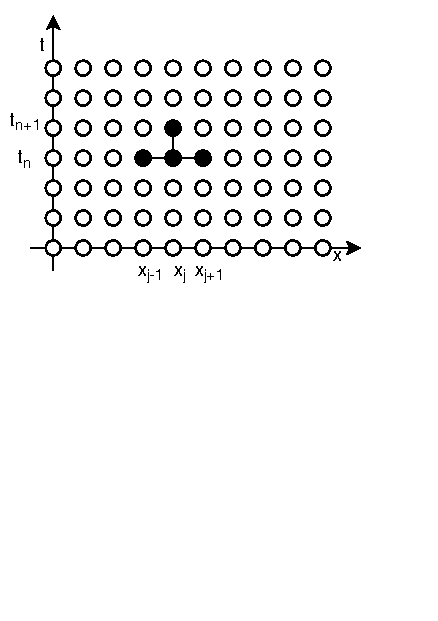
\includegraphics[width=0.5\linewidth, trim={0 5cm 0 0}]{Figures/FTCS}
    \caption[FTCS stencil]{Points used in the FTCS method}
    \label{fig:FTCSmesh}
\end{figure}


Now for the diffusion term, the most obvious approximation is to apply the forward difference scheme twice.
\begin{align*}
\partial_{xx} u(t_n,x_j) &\approx \partial_x \left(\frac{U^n_{j+1}- U^n_j}{\Dx}\right)\\
&=  \left(\frac{\partial_x U^n_{j+1} - \partial_x U^n_j}{\Dx}\right)\\
&\approx \frac{U^n_{j+1} - 2U^n_{j} + U^n_{j-1}}{(\Dx)^2}
\end{align*}
This is sufficient to give a first approximation to \eqref{eq:heat}.
\begin{align}\label{eq:FTCSheat}
\frac{U^{n+1}_j- U^n_j}{\Dt} &= \sigma \frac{U^n_{j+1} - 2U^n_{j} + U^n_{j-1}}{(\Dx)^2}\\
U^{n+1}_j &= U^n_j +  \frac{\sigma\Dt}{(\Dx)^2}\lbrack U^n_{j+1} - 2U^n_{j} + U^n_{j-1}\rbrack 
\end{align}
This is the Forward Time Centred Space (FTCS) method, a fully explicit scheme which means that we can write the next time step solely in terms of known values. We now have a method for approximating the true solution. When developing any numerical scheme, three properties need to be considered: stability, consistency and convergence. These concepts will be developed further below. Heuristically, a scheme is unstable if certain mesh spacings cause rapid growth in solutions -- a blow-up. A method is consistent if the error it makes in each step tends to zero as the size of the step tends to zero. Finally, a scheme is convergent if the approximate solution tends towards the true solution for any point in space and time. 

The heat equation \eqref{eq:heat} can be solved by separation of variables, giving the solution as a Fourier series. If the initial data is a single Fourier mode, the solution is
\begin{align*}
&u(t,x) = \mathrm{e}^{-\sigma(2\pi k)^2 t} \phi_k(x), && \phi_k(x) = \mathrm{e}^{2\pi i k x} \text{ for } k \in \mathbb{Z}.
\end{align*} 
If we assume our approximate solution is a Fourier mode, a criterion for stability will emerge.
\begin{align}
&U^n_j = \lambda^n \mathrm{e}^{ik(j\Dx)}, \qquad k \in \mathbb{Z} \label{eq:fouriermode}\\
\implies &U^{n+1}_j = \lambda U^n_j, \qquad U^n_{j\pm 1} = \mathrm{e}^{\pm ik\Dx}U^n_j \notag \\
\end{align}
Clearly if $|\lambda|>1$, the solution will be unstable. Substituting this into the finite difference scheme \eqref{eq:FTCSheat} gives
\begin{equation}\label{eq:FTCSlambda}
\lambda = 1 - 4\mu \sin^2\left(\frac{k\Dx}{2}\right), \qquad \text{ with } \mu = \frac{\sigma \Dt}{(\Dx)^2},
\end{equation}
and so,
\[
U^n_j = \left(1 - 4\mu \sin^2\left(\frac{k\Dx}{2}\right)\right)^n\mathrm{e}^{ikj\Dx}.
\]
Looking at \eqref{eq:fouriermode}, as $n \to \infty$, the numerical solution will grow unless $|\lambda|\leq 1$. If  $|\lambda|\leq 1$, the solution will decay with higher modes being damped quicker. This is what we expect from our analytic knowledge of the heat equation. The restriction on the mesh spacing thus arises from \eqref{eq:FTCSlambda}, 
\begin{align*}
-1 \leq \lambda \leq 1 \implies  \mu = \frac{\sigma \Dt}{(\Dx) ^2} \leq \frac{1}{2}
\end{align*}
This is not ideal: if more accuracy is required in the solution we can refine the space mesh, however in doing so the time step must also be shortened to maintain stability and the computational effort quickly increases.


The error made in each time step is the local truncation error, $R$, of the scheme. The local truncation error is the residual obtained by substituting the exact solution $u(t,x)$ into the discretisation. Performing a Taylor expansion around $t = n\Dt$ gives
\begin{align*}
&u^{n+1}_j = u^n_j + \Dt \partial_t u^n_j + \frac{1}{2}(\Dt)^2 \partial_{tt} u^n_j + \mathcal{O}(\Dt^3)\\
\implies& \frac{u^{n+1}_j - u^n_j}{\Dt}= \partial_t u^n_j + \frac{1}{2}\Dt \partial_{tt} u^n_j + \mathcal{O}(\Dt^2).
\end{align*}

And similarly around $x=j\Dx$,
\begin{align*}
&u^n_{j+1}=  u^n_j + \Dx \partial_x u^n_j + \frac{1}{2}(\Dx)^2 \partial_{xx} u^n_j + \frac{1}{3!}(\Dx)^3 \partial_{xxx} u^n_j + \frac{1}{4!}(\Dx)^4 \partial_{xxxx} u^n_j +  \mathcal{O}(\Dx^5)\\
\implies& \frac{u^n_{j+1} -2  u^n_j + u^n_{j-1}}{\Dx^2}  = \partial_{xx}u^n_j + (\Dx)^2u_{xxx} + \mathcal{O}(\Dx^3).
\end{align*}  
The local truncation error is then
\begin{align*}
&R^n_j = \underbrace{\partial_t u^n_j - \sigma \partial_{xx}u^n_j}_{=0} +\mathcal{O}(\Dt)+ \mathcal{O}(\Dx^2)\\
\implies& R^n_j = \mathcal{O}(\Dt)+\mathcal{O}(\Dx^2).
\end{align*}
The first two terms are zero as $u$ is solves the heat equation. The explicit scheme \eqref{eq:FTCSheat} is then first order in time and second order in space. 

\begin{figure}
    \centering
    \begin{minipage}[b]{0.49\textwidth}
        \centering
        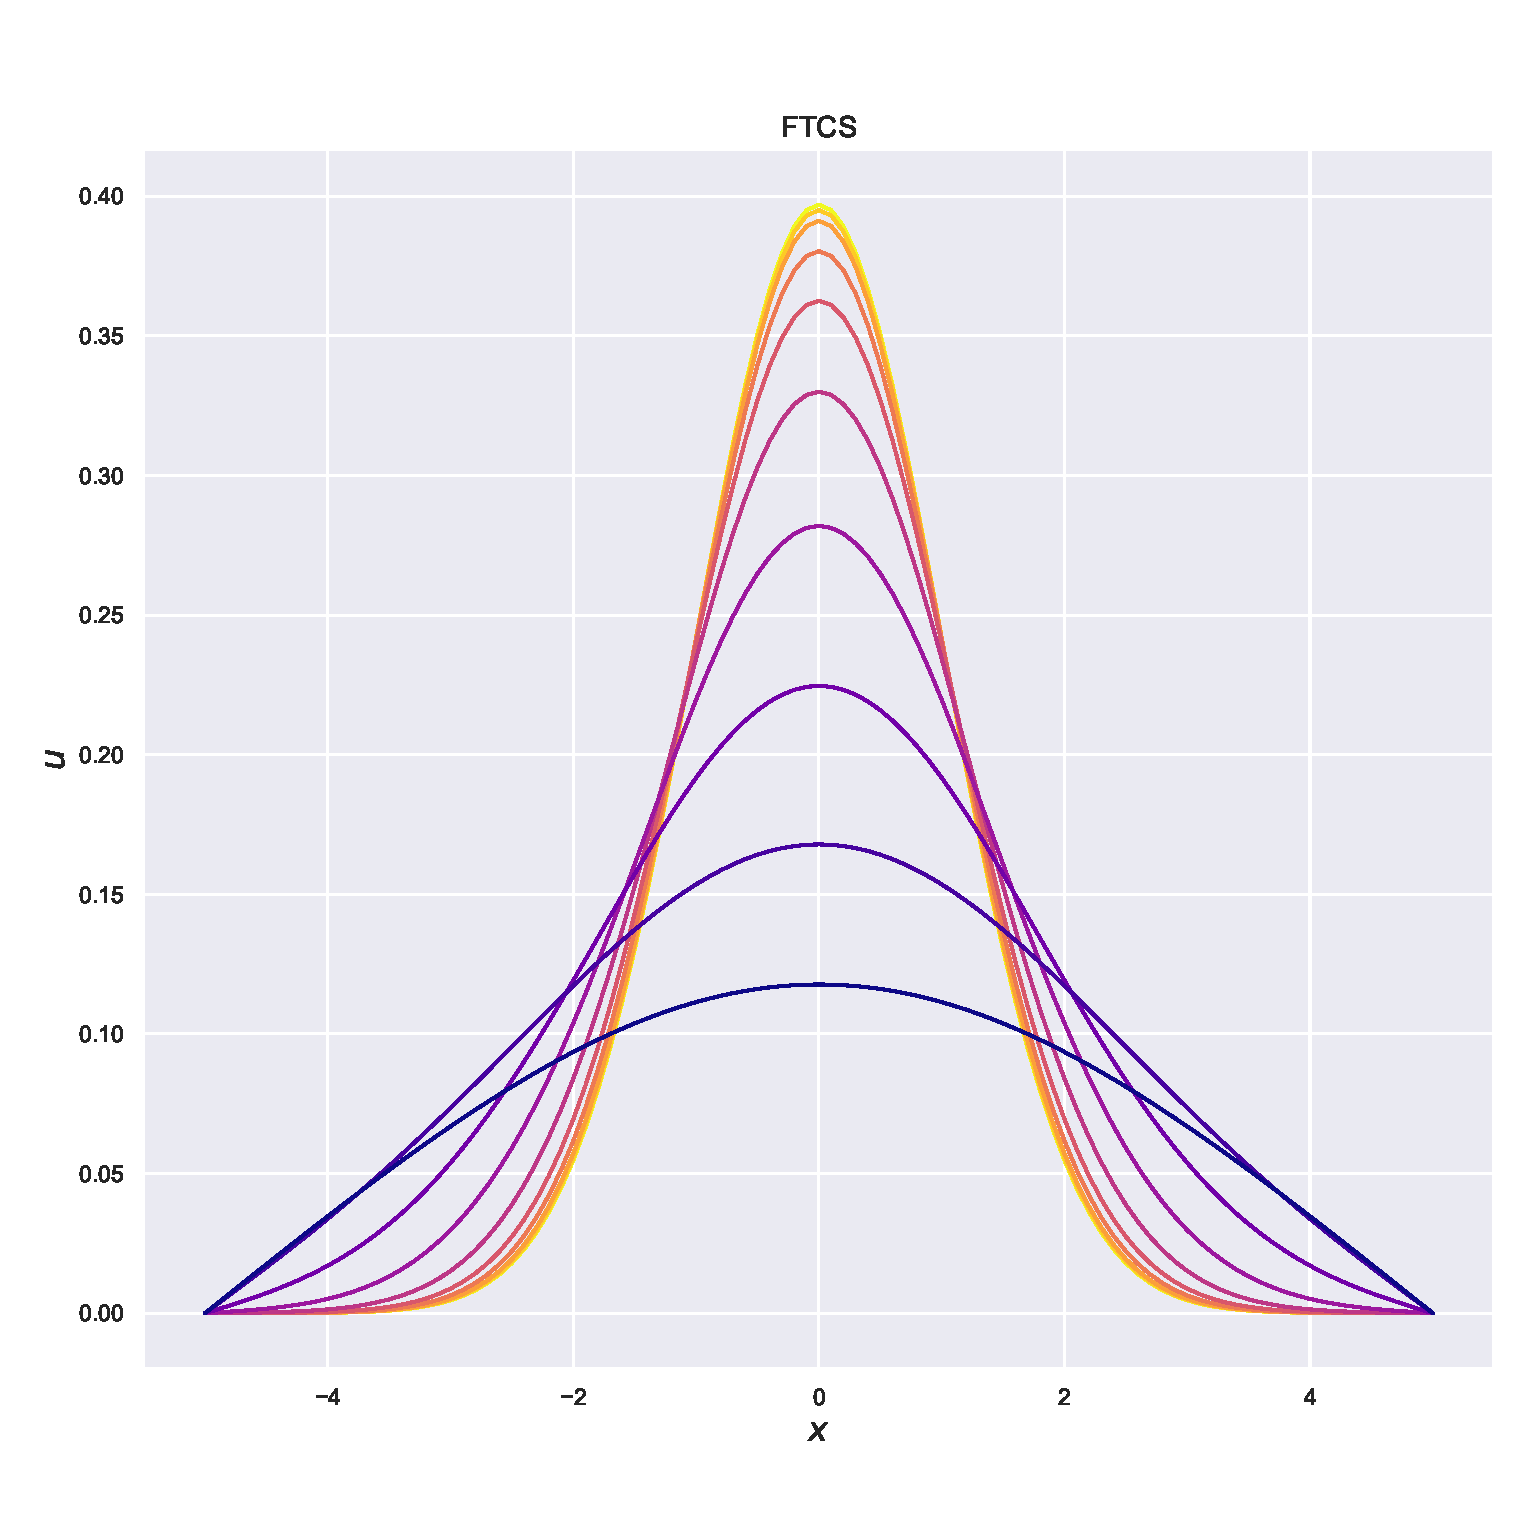
\includegraphics[width=\textwidth]{Figures/stableFTCSheat.eps}
        \subcaption{\(\Delta t = 0.005\)}
    \end{minipage} %
    \begin{minipage}[b]{0.49\textwidth}
        \centering
        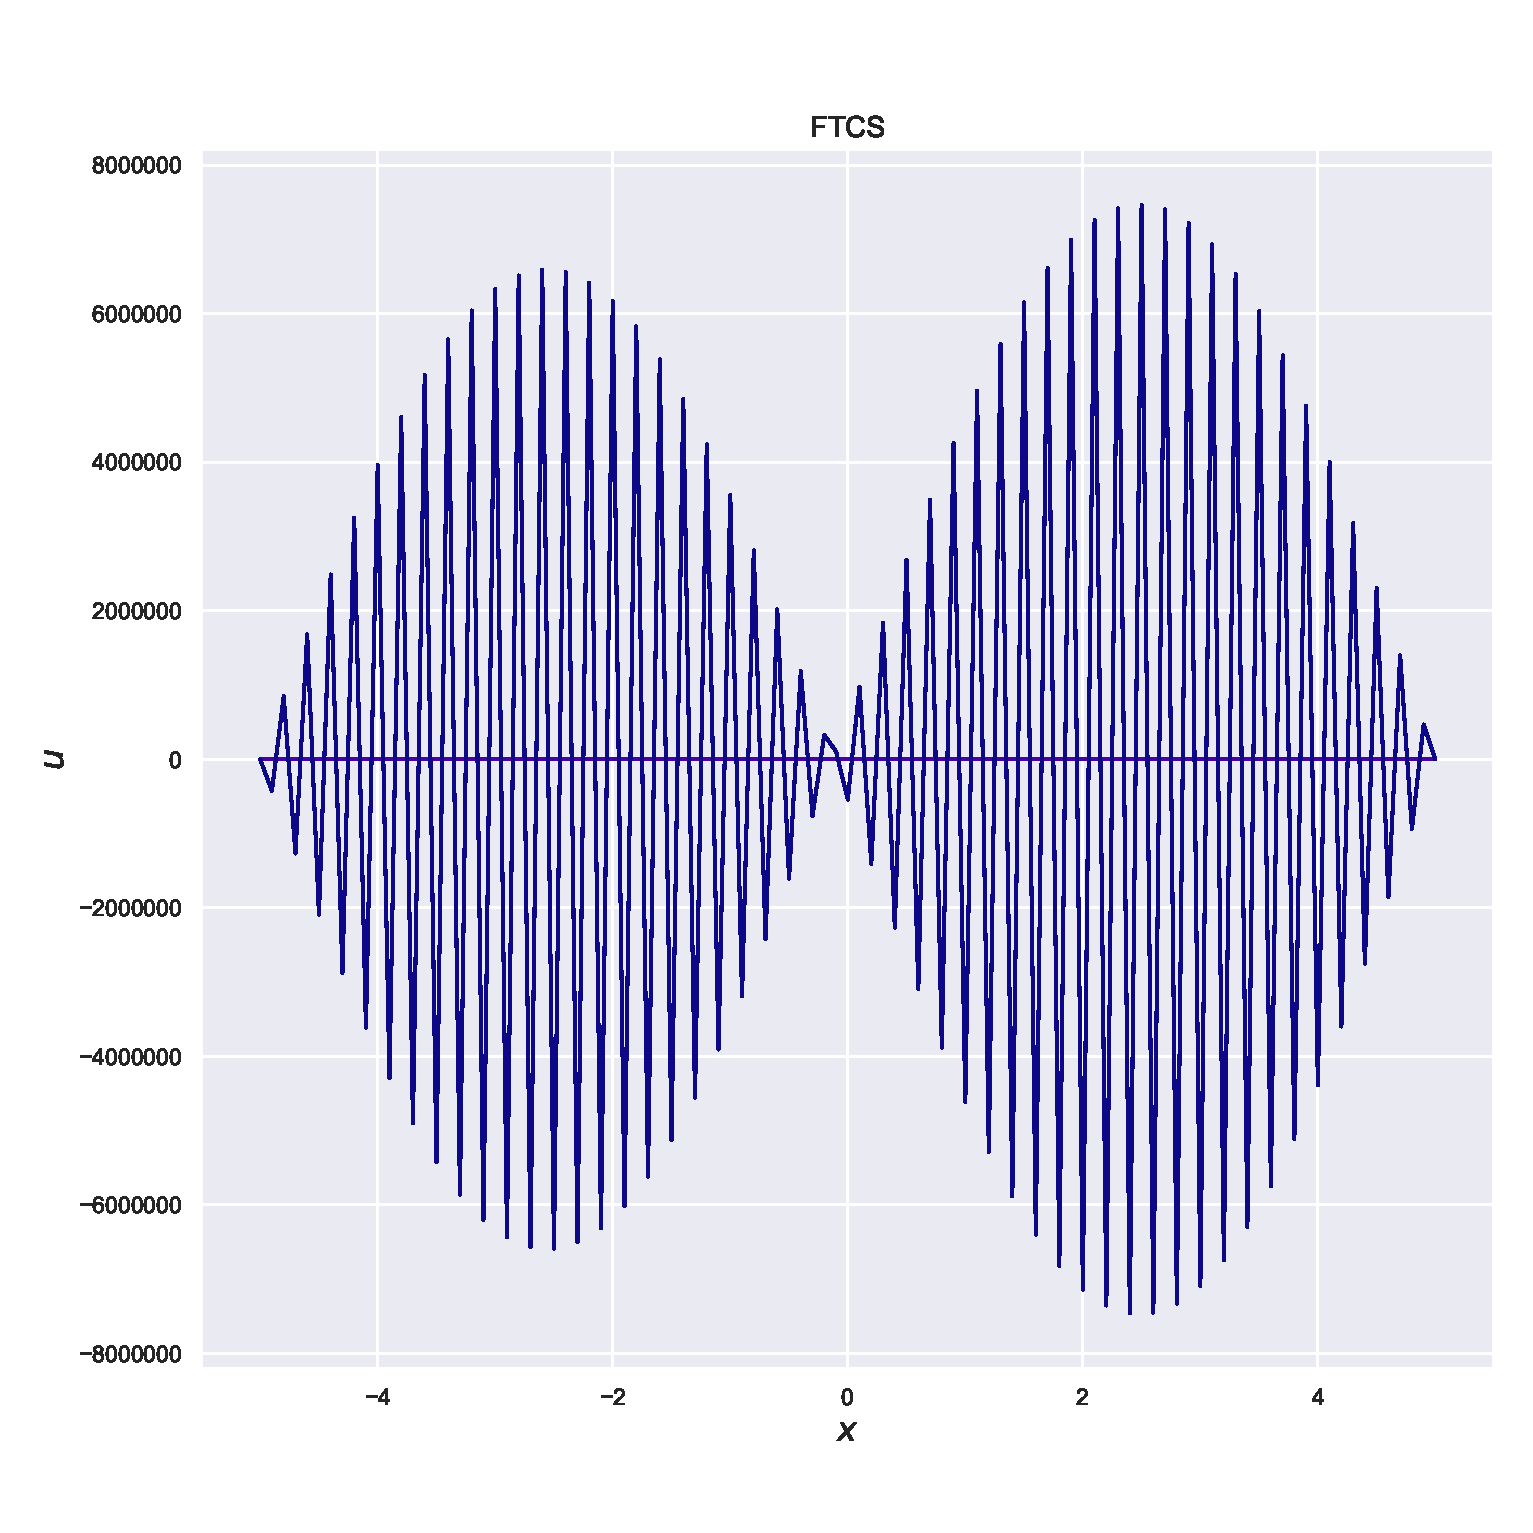
\includegraphics[width=\textwidth]{Figures/unstableFTCSheat.eps}
        \subcaption{\(\Delta t = 0.0051\)}
    \end{minipage} %
    \caption[Instability in the FTCS scheme]{Using the \texttt{FTCS} scheme to solve the heat equation \eqref{eq:heat} on \( \lbrack -5,5\rbrack \times\lbrack -1,1\rbrack\) with \(\sigma =1, \Delta x = 0.1\) with a Gaussian initial profile. When the stability condition is violated, $\lambda>1$ and the solution grows exponentially.} 
    \label{fig:FTCSunstable}
\end{figure}

A numerical scheme is consistent if the local truncation error tends to zeros as \(\Dx, \Dt \to 0\). The FTCS scheme is consistent of order one in time and two in space and stable so long as \(\mu \leq \frac{1}{2}\).  A scheme is convergent if for any fixed point  \((x^*,t^*) \in [-L,L] \times [0,T]\), \[x_j \to x^*, t_n \to t^* \implies U^n_j \to u(x^*,t^*).\]
The explicit scheme is convergent when it is stable. The stability condition is a great drawback of the FTCS method. In the next section we look to new methods to remove any restrictions on the mesh spacing, whilst maintaining (or improving) the truncation error.

\subsubsection*{Backward Time Centred Space}
If instead of looking at the forward time difference we look at the backward time difference, the scheme becomes stable. This is surprising, very little appears to change but the scheme is fundamentally different. This method is implicit, meaning that its solution requires a more complex calculation at every time step. However, the lack of restriction on the size of the timestep means fewer steps (and therefore fewer calculations) need to be performed. The backward time centred space (BTCS) scheme for \eqref{eq:heat} is
\begin{align}
\frac{U^{n+1}_j- U^n_j}{\Dt} &= \sigma \frac{U^{n+1}_{j+1} - 2U^{n+1}_{j} + U^{n+1}_{j-1}}{(\Dx)^2}.
%\label{eqBTCSheat}
\end{align}
The only difference here is the right hand side is calculated at the $n+1^{\text{th}}$ time step whereas in the FTCS algorithm it is taken at $n$. This scheme cannot be written explicitly in terms of known values, that is, the $n^{\text{th}}$ time step. Instead, we move all unknowns to the left hand side to give
\[
-\mu U^{n+1}_{j-1} + (1+2\mu)U^{n+1}_j - \mu U^{n+1}_{j+1} = U^n_j
\]
where, as before, $\mu=\frac{\Dt}{(\Dx)^2}$. This leads to a set of $J-1$ simultaneous equations. As the system is tridiagonal, the Thomas algorithm can be used to efficiently solve the system. See Appendix \ref{app:thomas} for a description.

The stability and consistency of the BTCS scheme can be found using the same techniques as was used for the explicit FTCS scheme. Assuming once again that the approximate solution as a Fourier mode, one obtains
\[\lambda = \frac{1}{1+4\mu \sin^2(\frac{1}{2}k\Dx)}.\]
This is less than one for any positive $\mu$, and so the BTCS method is unconditionally stable. The local truncation error of the scheme is the same as that of the FTCS method, namely the BTCS scheme is first order in time and second order in space. We now have a method with the same accuracy as the explicit scheme, but with no restriction on mesh size. The final method introduced will maintain this lack of constraint whilst increasing the accuracy, with little extra effort.
\begin{figure}
    \centering
    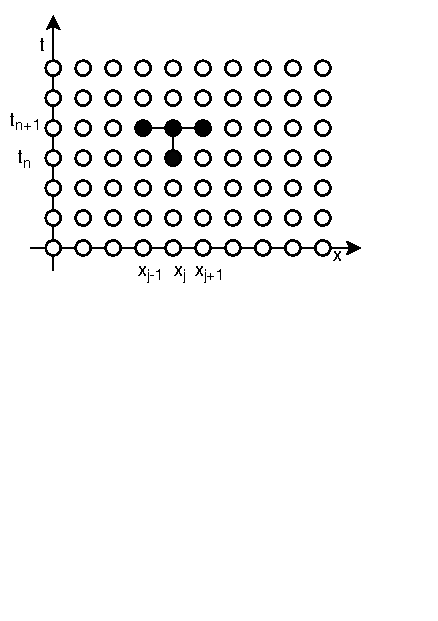
\includegraphics[width=0.5\linewidth, trim={0 5cm 0 0}, clip]{Figures/BTCS}
    \caption[BTCS stencil]{The points used in the implicit BTCS scheme}
    \label{fig:BTCSmesh}
\end{figure}

\subsubsection*{Theta Method}
So far we have considered two methods, each using a set of three points to update. Given that we know how to solve implicit and explicit methods is there an optimal hybrid between the two? The theta method aims to find this optimum by taking a weighted average of the FTCS and BTCS schemes. Applied to our toy problem \eqref{eq:heat}, the scheme is
\[
\frac{U^{n+1}_{j}-U^{n}_{j}}{\Dt} = \sigma\left(\theta \frac{U^{n+1}_{j+1}-2U^{n+1}_{j}+U^{n+1}_{j-1}}{(\Dx)^2}+(1-\theta)\frac{U^{n}_{j+1}-2U^{n}_{j}+U^{n}_{j-1}}{(\Dx)^2}\right),
\]
where $0\leq \theta 1$ is a weighting parameter. For $\theta = 0$, the FTCS scheme is recovered, and likewise when $\theta = 1$ the scheme is just the BTCS method. The aim of this section is to find an optimum weight for $\theta$, if one exists. Optimum here means the value that decreases the truncation error the most, whilst maintaining the unconditional stability of the BTCS method. Rearranging as a tridiagonal system gives
\[
-\theta\mu U^{n+1}_{j-1} + (1+2\theta\mu)U^{n+1}_j - \theta\mu U^{n+1}_{j+1} = U^n_j + (1-\theta)\mu \left[U^n_{j+1} - 2U^n_{j} + U^n_{j-1} \right]. 
\]

Using the stability analysis from the FTCS scheme, one obtains
\[ \lambda = \frac{1-4(1-\theta)\mu\sin^2(\frac{1}{2}k\Dx)}{1+4\theta\mu\sin^2(\frac{1}{2}k\Dx)}.\]
Note again that if $\theta = 1$, $\lambda$ is as it was for the BTCS scheme, and if $\theta = 0$, the value for the FTCS method is recovered. This is always less than one and is greater than minus one if
\[\mu(1-2\theta) \leq \frac{1}{2}.\]
Hence any choice of $\theta \geq \frac{1}{2}$ is sufficient for unconditional stability. This makes intuitive sense: the BTCS method is unconditionally stable, so any weighting preferring this scheme is also stable. If $\theta > \frac{1}{2}$, the mesh spacing can be adjusted to retain stability, as in the FTCS method. 
\begin{figure}
    \centering
    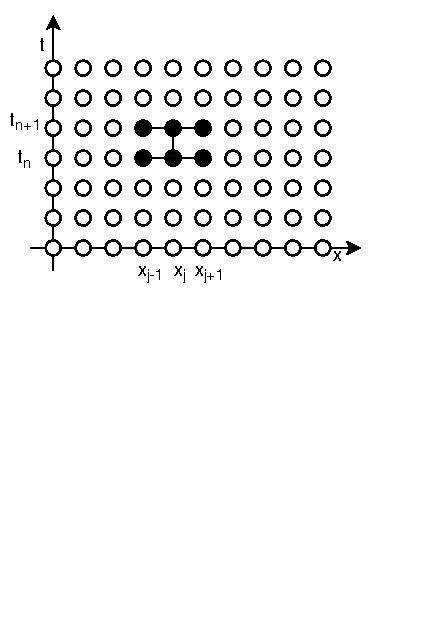
\includegraphics[width=0.5\linewidth, trim={0 5cm 0 0}, clip]{Figures/CN}
    \caption[Theta Method Stencil]{Points used in the Theta method}
    \label{fig:CNmesh}
\end{figure}
Thus far there is no reason to prefer the theta method over the simpler BTCS scheme. However, let's consider the truncation error of the scheme using similar analysis as above, expanding this time around the midpoint of the mesh, $(x_j, t_{n+\frac{1}{2}})$.
    \[\begin{split}R^{n+\frac{1}{2}}_j = \lbrack \partial_t u - \partial_{xx}u\rbrack &+ \left[\left(\frac{1}{2} - \theta\right)\Dt \partial_{xxt}u - \frac{1}{12}(\Dx)^2\partial^4_{x} u\right]\\&+\left[\frac{1}{24}(\Dt)^2\partial^3_{t}u - \frac{1}{8}(\Dt)^2u_{xxtt}\right]\\
    &+\left[\frac{1}{12}\left(\frac{1}{2}-\theta\right)\Dt (\Dx)^2\partial_{xxxxt}u - \frac{2}{6!}(\Dx)^4\partial^6_xu\right]
    \end{split} \]
So for arbitrary choice of $\theta$, the scheme remains first order in time and second order in space. However, if $\theta=\frac{1}{2}$, the first order in time term is zero, and the scheme is second order in both time and space. The optimal value of $\theta$ is the even weighting of the FTCS and BTCS scheme. This method is known as the Crank-Nicolson (CN) method, and is the first choice when using finite difference methods -- it is simple, quick and accurate to second order. Table \ref{tab:FDmethods} summarises the results of this section. The supplementary notebook contains all three solvers for the heat equation \eqref{eq:heat}. For the model, a Crank-Nicolson scheme will be used.
\begin{table}
    \centering
    \begin{tabular}{|c|c|c|c|}
        \hline
        & & & \\[-0.5em] 
        Method & FTCS ($\theta=0$) & BTCS ($\theta=1$) & Crank-Nicolson ($\theta=\frac{1}{2}$) \\[0.3em] 
        \hline 
        & & & \\[-0.5em] 
        LTE & $\mathcal{O}(\Dt), \mathcal{O}(\Dx^2)$ & $\mathcal{O}(\Dt), \mathcal{O}(\Dx^2)$ & $\mathcal{O}(\Dt^2), \mathcal{O}(\Dx^2)$ \\[0.3em]  
        \hline
        & & & \\[-0.5em]  
        Stablity Condition & $\mu\leq \frac{1}{2}$ & None & None \\[0.3em]  
        \hline 
        & & & \\[-0.5em] 
        Explicit/Implicit & Explicit & Implicit & Implicit \\[0.3em]  
        \hline 
    \end{tabular}
\caption{Finite difference methods for diffusion equations}
\label{tab:FDmethods}
\end{table}

\begin{figure}
    \centering
    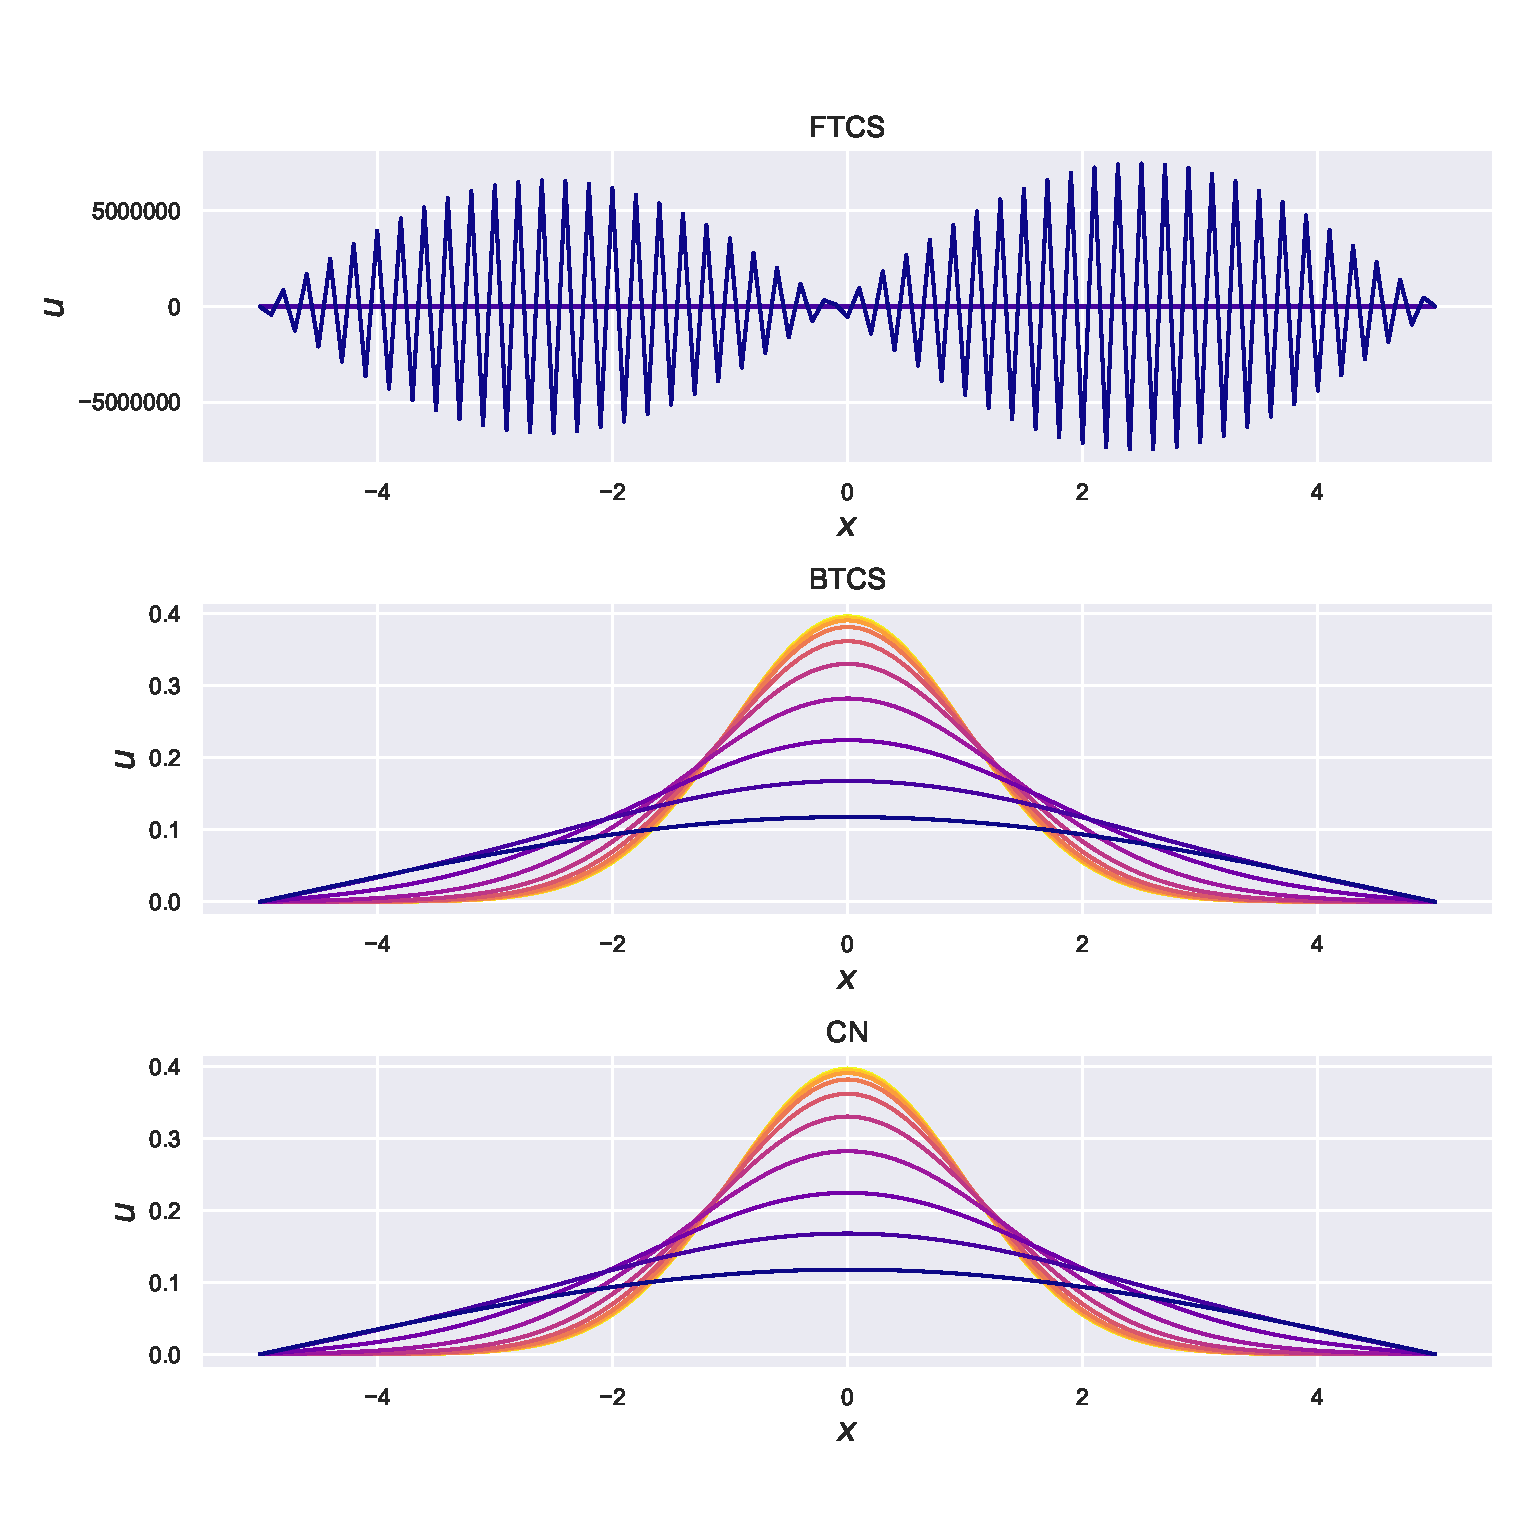
\includegraphics[width=0.7\linewidth]{Figures/FTCSandCN}
    \caption[Comparison of FTCS, BTCS, CN solvers]{Solving the heat equation as in Figure \ref{fig:FTCSunstable} using FTCS, BTCS and CN solvers respectively. The implicit solvers remain stable regardless of step size, and return an accurate solution.}
    \label{fig:ftcsandcn}
\end{figure}
\subsection{Advection Equations}
Our prototypical example in this case will be the one-way wave equation,
\begin{equation}\label{eq:wave}\begin{cases}
\partial_t u(t,x) + a(x)\partial_x u(t,x)=0,\\
u(0,x) = u_0(x),  &t\in\R^+, x\in\R.
\end{cases}\end{equation}
Advection equations are, in general, much more difficult to solve numerically than the diffusion equation. In this section we will consider $a$ constant to illustrate the methods. When solving an advection equation numerically, any scheme must satisfy the CFL condition. To motivate the choice of scheme, we first introduce this condition.

The exact solution to an advection equation can be found by using the method of characteristics. Characteristics are lines on which the PDE \eqref{eq:wave} reduces to an ODE. Let 
\[\od{x}{t} = a(x,t).\]
Then using the chain rule,
\[
\od{u}{t} = \partial_t u +\od{x}{t}\partial_x u = 0,
\]
as $u$ solves the PDE. Thus on a characteristic, the solution is constant. For the case when $a$ is constant, the characteristics are the straight lines $x-at = const.$ and the solution is \[ u(x,t) = u_0(x-at).\] The initial profile is simply transformed at a speed $a$. The solution at a point $(x_j,t_n)$ is then obtained by finding the characteristic through this point and following it backwards in time to $t=0$. If a discretisation is applied to equation \eqref{eq:wave}, we obtain the explicit scheme
\[\frac{U^{n+1}_j-U^n_j}{\Dt} =-a \frac{U^n_{j+1}-U^n_j}{\Dx}.\] 
As in the FTCS method, to find the value of the solution at the next time point we evaluate
\[U^{n+1}_j = U^n_j - c(U_{j+1}-U_j), \]
where $c=\frac{a\Dt}{\Dx}$. Figure \ref{fig:CFL} shows the dependence of the current point on all previous points. Each point depends on two points from the previous time level, propagating all the way back to the initial line. This set of points, here a triangle, is the domain of dependence of the scheme. The CFL condition states that for a scheme to converge the characteristic curve passing through a point must stay within the domain of dependence for that point. In Figure \ref{fig:CFL}, two example characteristics are plotted for $a>0 (PQ)$ and for $a<0 (PR)$. The explicit scheme outlined above is then only convergent for negative values of $a$, otherwise the characteristic lies outside of the domain of dependence. Intuitively, a scheme cannot be accurate if it cannot `see' the wave arriving. If the wave is moving too fast, the CFL condition may be violated as the characteristic becomes much shallower and again lies outside the domain of dependence of the numerical scheme. This can be counteracted by reducing the timestep, effectively widening the base of the domain of dependence until it includes the characteristic. For this scheme this requires 
\[c =\frac{a\Dt}{\Dx} < 1.\]
\begin{figure}
    \centering
    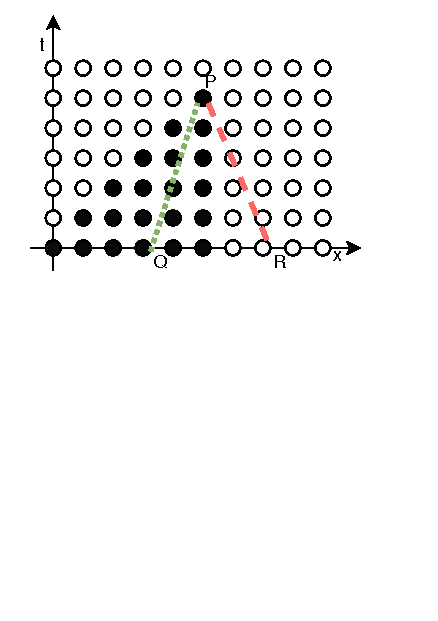
\includegraphics[width=0.7\linewidth, trim={0 5cm 0 0}, clip]{Figures/CFL}
    \caption[CFL Condition]{}
    \label{fig:CFL}
\end{figure}
This condition ensures the solution does not travel further in one time step than one spacestep, thereby remaining in the domain of dependence. This condition is dependent on the geometry of the domain of dependence. The CFL condition is necessary but not sufficient for stability, as the following scheme shows. One way to satisfy the condition would be to make the triangle isosceles instead of right-angled. This can be achieved by taking a central difference in space:
\[
    \frac{U^{n+1}_j-U^n_j}{\Dt} =-a \frac{U^n_{j+1}-U^n_{j-1}}{\Dx}
\]
The CFL condition here requires $|a|\frac{\Dt}{\Dx} < 1$. By applying the stability analysis used for the FTCS method, one obtains $\lambda = 1-c i \sin(k\Dx)$. This is always greater than one, and the scheme is thus unconditionally unstable, despite satisfying the CFL condition. The upwind scheme is the simplest stable method for advection equations. It switches the direction of the difference based on the direction of the wave, thereby always `facing into the wave' (upwind).
\[
U^{n+1}_{j} = \begin{cases} U^{n}_{j}-c(U^{n}_{j+1}-U^{n}_{j}) & \text{ if } a<0\\[0.5em]
U^{n}_{j}-c(U^{n}_{j}-U^{n}_{j-1}) & \text{ if } a>0\\
\end{cases}
\]
Satisfying the CFL condition here requires $|a|\frac{\Dt}{\Dx} < 1$, and in fact stability analysis shows this is also sufficient for stability. Furthermore, the local truncation error can be calculated. Here we set $a>0$.
\begin{align*}
    R^n_j &= \frac{u^{n+1}_j-u^n_j}{\Dt}  + a \frac{u^n_{j}-u^n_{j-1}}{\Dx}\\
    &=\frac{1}{2}(\Dt \partial^2_t u - a\Dx \partial^2_x u)+\dots
\end{align*}
So the upwind scheme is first order in both time and space. Higher order schemes are available for advection equations, however this will suffice for a first approximation to the model. There are problems, however, with artificial dissipation in this scheme, as Figure \ref{fig:advection} shows. For a heuristic insight, we can consider the modified equation. By a Taylor expansion in the upwind scheme, we obtain
\[\frac{u^n_j - u^n_{j-1}}{\Dx} = \partial_x u^n_j + \frac{1}{2}\Dx\partial^2_{x}u^n_j + \mathcal{O}(\Dx^2). \]
This shows that the numerical solution will be more closely approximating an advection-diffusion equation:
\[\tilde{u}_t + a\tilde{u}_x = \frac{1}{2}a\Dx\partial^2_x \tilde{u}.\]
The modified equation shows the source of the dissipative effects seen in the scheme.
\begin{figure}
    \centering
    \begin{minipage}[b]{0.49\textwidth}
        \centering
        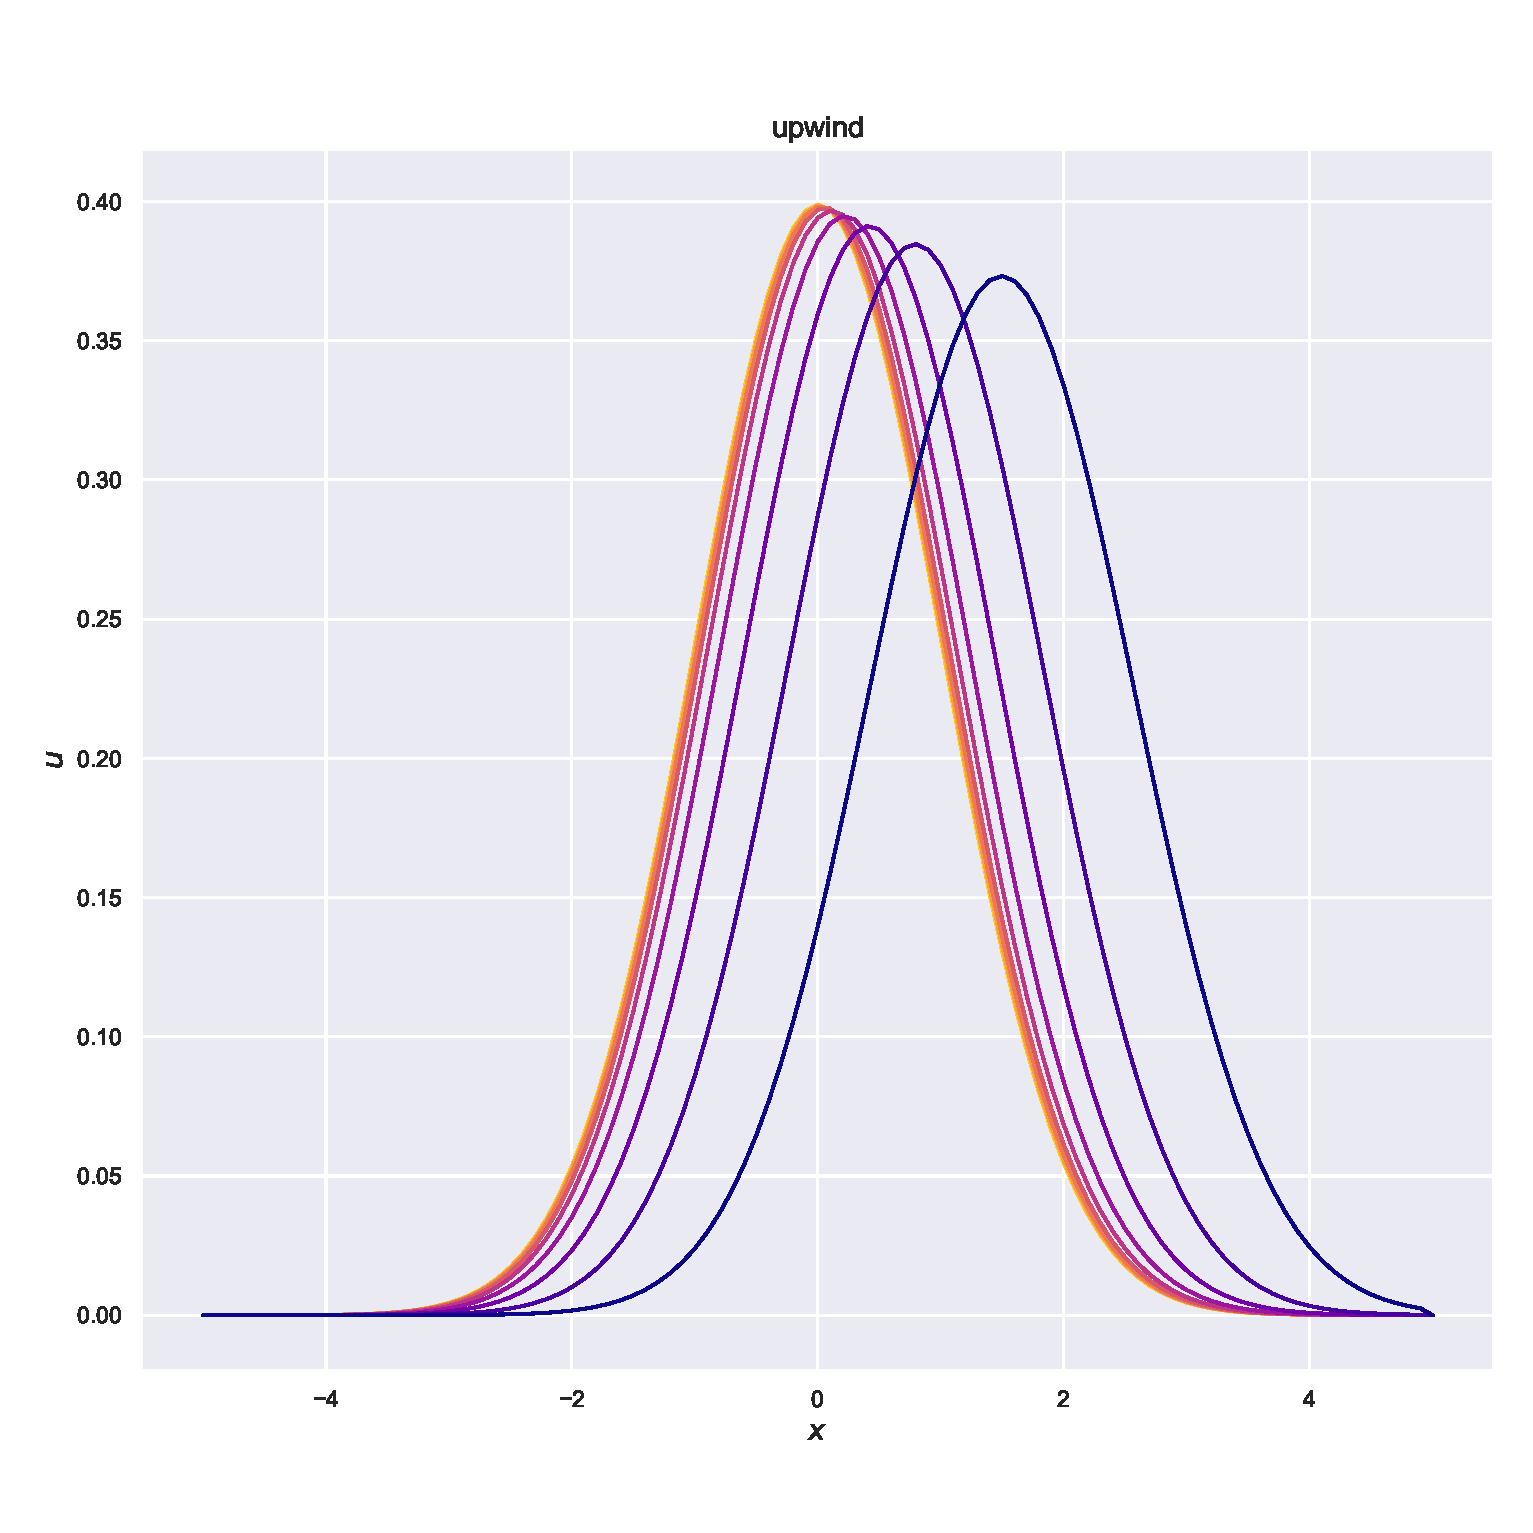
\includegraphics[width=\textwidth]{Figures/advgaussian.eps}
        \subcaption{$U_0 \sim \mathcal{N}(0,1)$}
    \end{minipage} %
    \begin{minipage}[b]{0.49\textwidth}
        \centering
        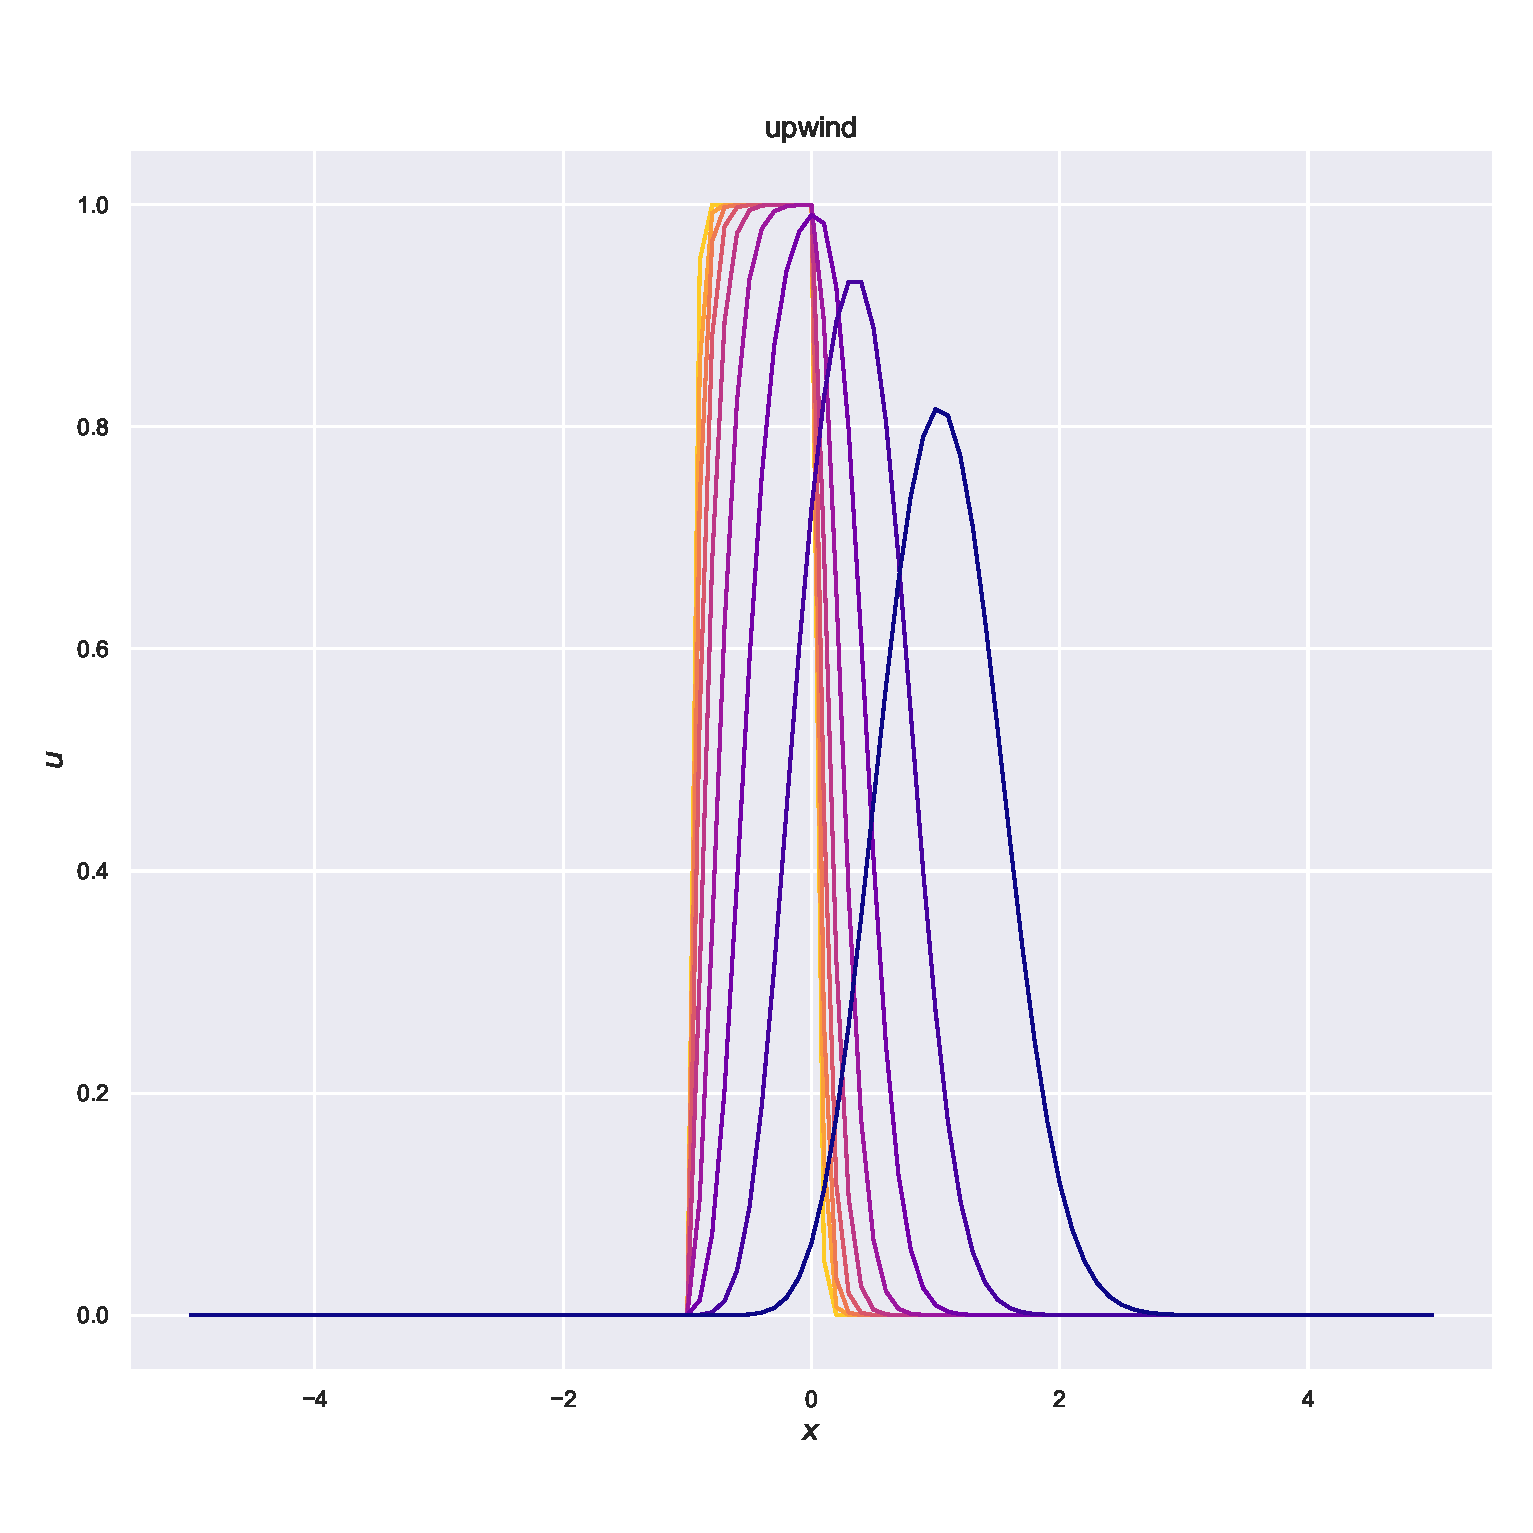
\includegraphics[width=\textwidth]{Figures/advindicator.eps}
        \subcaption{$U_0(x) = \mathbbm{1}_{\lbrack-1,0\rbrack}(x)$}
    \end{minipage} %
    \caption{Solving equation \eqref{eq:wave} with the upwind scheme. Even with very smooth initial data, dissipative effects can be severe.} 
    \label{fig:advection}
\end{figure}
\subsubsection*{Finite Volume Schemes}
One aspect of the advection equation \eqref{eq:wave} the schemes thus far have not yet exploited is its conservation of mass. Finite volume methods ensure mass is conserved in the scheme, something not yet considered that can be a source of error. Finite volume schemes can be applied to any conservation (or continuity) equation. A conservative equation is one that can be written in the form
\[\partial_t u + \partial_x(a(x) u).\]
On the same mesh as previously, auxiliary points are introduced between points in space, namely $x_{j+\frac{1}{2}}$ for $0\geq j \leq J-1$. Within any interval (or volume), $\Omega_j = \left[x_{j-\frac{1}{2}},x_{j+\frac{1}{2}}\right]$, we can calculate the average density.
\[\bar{u}(x_j) = \frac{1}{\Dx}\int_{\Omega_j} u(x) \dif x = u(x_j) + \frac{(\Dx)^2}{24}\partial^2_x u(x_j) +\dots \]

Furthermore, the change in the average density within the cell is equal to difference of the mass lost through the boundary of the volume, that is,
\[
\Dx\od{\bar{u}(x_j)}{t} = a(x_{j-\frac{1}{2}})u(x_{j-\frac{1}{2}}) - a(x_{j-\frac{1}{2}})u(x_{j-\frac{1}{2}}), 
\]
This is also known as the flux across the boundary. A finite volume scheme balances fluxes across the domain, thereby maintaining total mass. Doing so leads to the first-order upwind scheme in flux form,
\[
\frac{U^{n+1}_j - U^n_j}{\Dt} = \frac{-1}{\Dx}\left[ a(x_{j+\frac{1}{2}})U^n_{j+\frac{1}{2}} - a(x_{j-\frac{1}{2}})U^n_{j-\frac{1}{2}}\right].  
\]
The value of $a$ at the midpoint is chosen to be the average of its value at the cell centres, that is $a(x_{j+\frac{1}{2}}) = \frac{1}{2}\left(a(x_j)+a(x_{j+1})\right)$. The scheme as written will be unstable if $a(x)<0$, for the same reason as in the previous section. The spatial bias needs to be changed depending on the direction of the wave. 
\[
a(x_{j+\frac{1}{2}})U^n_{j+\frac{1}{2}} = a^+(x_{j+\frac{1}{2}})U^n_{j} + a^-(x_{j+\frac{1}{2}})U^n_{j+1},
\]
where $a^+ = \max(a,0), a^- = \min(a,0)$.  This scheme is still order 1, however it provides the ideal setting for developing higher order schemes.